\documentclass[12pt, a4paper]{article}

\usepackage[utf8x]{inputenc}
\usepackage[greek, english]{babel}
\usepackage{caption}
\usepackage[section]{placeins}
\usepackage{balance}
\usepackage{dblfloatfix}
\usepackage{hyperref}
\usepackage{color}
\usepackage{graphicx}
\usepackage{float}

%\usepackage[margin=2cm]{geometry}
%\usepackage{graphicx,wrapfig,lipsum}

\newcommand{\en}{\selectlanguage{english}}
\newcommand{\gr}{\selectlanguage{greek}}

\hypersetup{
	colorlinks=true,
	linkcolor=blue,
	filecolor=magenta,
	urlcolor=blue,
}

\begin{document}
	
\gr
\begin{titlepage}
	
	\begin{center}
		\vspace*{0.5cm}
		
		\LARGE
		\textbf{\gr ΠΜΣ ΕΠΙΣΤΗΜΗ ΚΑΙ ΜΗΧΑΝΙΚΗ ΔΕΔΟΜΕΝΩΝ}
		
		\vspace{0.5cm}
		%\LARGE
		\Large 
		\gr{ΑΥΤΟΜΑΤΗ ΚΑΤΑΤΜΗΣΗ ΚΑΙ ΚΑΤΗΓΟΡΙΟΠΟΙΣΗ ΤΗΣ ΠΟΛΥΔΙΑΣΤΑΤΗΣ ΧΡΟΝΟΣΕΙΡΑΣ ΑΙΣΘΗΤΗΡΙΑΚΩΝ ΣΗΜΑΤΩΝ}
		
		\vspace{1.5cm}
		
		\textbf{Γεώργιος Βαρδάκας}
		
		\vfill
		
\includegraphics[width=0.5\textwidth]{logo.png}
		
		\textbf{Υπεύθυνος Καθηγητής: \\Παρσόπουλος Κωνσταντίνος}
		\vfill
		
		%\bf{Τρίτη εργασία του μαθήματος της Βελτιστοποίησης Ακ.έτους 2020-2021}\\
		
		
		\vspace{0.8cm}
		
		\Large
		Τμήμα Μηχανικών Η/Υ και Πληροφορικής\\
		Πολυτεχνική Σχολή Πανεπιστημίου Ιωαννίνων\\
		%Ελλάδα\\
		\date{\today}
		
	\end{center}
\end{titlepage}


\tableofcontents
\newpage

\gr
\section{Εισαγωγή}
Αυτόματη κατάτμηση και κατηγοριοποίηση της πολυδιάστατης χρονοσειράς αισθητηριακών σημάτων

\section{Συλλογή Δεδομένων}
Μία προαπαίτηση για την κατασκευή ενός μαθηματικού μοντέλου μηχανικής μάθησης είναι φυσικά τα δεδομένα, καθώς αυτές οι μέθοδοι μαθαίνουν μέσα από αυτά. Για την συλλογή των δεδομένων έγινε χρήση του έξυπνου ρολογιού \en Fitbit Versa\gr. Το έξυπνο αυτό ρολόι, μας δίνει την δυνατότητα να αντλήσουμε τις μετρήσεις που καταγράφουν οι διαθέσιμοι αισθητήρες του. Οι αισθητήρες αυτοί αποτελούνται από από το γυροσκόπιο, το επιταχυνσιόμετρο καθώς και τον αισθητήρα καρδιακών παλμών. Οι αισθητήρες του γυροσκοπίου και του επιταχυνσιομέτρου καταγράφουν μετρήσεις με συχνότητα $10$ \en H \gr ενώ ο αισθητήρας καρδιακών παλμών καταγράφει μετρήσεις με συχνότητα $1$ \en H\gr. Στην παρούσα εργασία έγινε χρήση μόνο των αισθητήρων του γυροσκοπίου και του επιταχυνσιομέτρου καθώς οι καταγραφές του αισθητήρα των καρδιακών παλμών δεν περιείχε χρήσιμη πληροφορία για την αυτόματη κατηγοριοποίηση της πολυδιάστατης χρονοσειράς των αισθητήρων. Συνολικά καταφέραμε να συλλέξαμε δεδομένα από εφτά διαφορετικούς χρήστες. Τα δεδομένα είναι μορφής πίνακα όπως ο παρακάτω:

\begin{figure}[H]
	\centering
	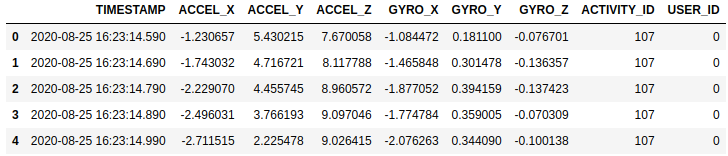
\includegraphics[width=1\textwidth, height=0.25\textheight]{Data.png}
	
	\caption{Πρώτες πέντε εγγραφές του πίνακας δεδομένων.}
	\label{plot:epoch-error}
\end{figure}
\noindent
όπου η κολόνα \en TIMESTAMP \gr αναφέρεται στο χρόνο δειγματοληψίας της εγγραφής, η κολόνα \en ACCEL\_\{X,Y,Z\} \gr αναφέρεται στην μέτρηση του επιταχυνσιομέτρου στον άξονα \{$x, y, z$\}, η κολόνα \en GYRO\_\{X,Y,Z\} \gr αναφέρεται στην μέτρηση του γυροσκοπίου στον άξονα \{$x, y, z$\}, η κολόνα \en ACTIVITY\_ID \gr δηλώνει την δραστηριότητα που πραγματοποιεί ο χρήστης και τέλος η κολόνα \en USER\_ID \gr αναφέρεται στον ποίος χρήστης έκανε την δραστηριότητα. Οι μετρήσεις των αισθητήρων καταγράφουν δείγματα στον τρισδιάστατο χώρο και αυτός είναι ο λόγος που κάθες αισθητήρας έχει τρεις μετρήσεις ($x, y, z$). Επίσης ο κάθε χρήστης έχει μοναδικό \en ID \gr.


\end{document}